\documentclass[10pt,a4paper]{article}
\usepackage[utf8]{inputenc}
\usepackage[spanish]{babel}
\usepackage{amsmath}
\usepackage{amsfonts}
\usepackage{amssymb}
\usepackage{makeidx}
\usepackage{graphicx}
\usepackage{lmodern}
\usepackage{kpfonts}
\usepackage{fourier}
\usepackage[hidelinks]{hyperref}
\usepackage[left=2cm,right=2cm,top=2cm,bottom=2cm]{geometry}
\author{Luis Angel Torres Pinto}
\title{Calcular los parámetros de circuitos de activación de transistores de potencia.}\\
\begin{document}
\maketitle
\centering

\includegraphics[scale=2]{upzmg.jpg}\\
\raggedright
\newpage 
\section{Transistor de Potencia }
El funcionamiento y utilización de los transistores de potencia es idéntico al de los transistores normales, teniendo como características especiales las altas tensiones e intensidades que tienen que soportar y, por tanto, las altas potencias a disipar.\\
\bigskip 
Existen tres tipos de transistores de potencia:\\

1.Bipolar\\
2.Unipolar o FET (Transistor de Efecto de Campo).\\
3.IGBT.\\
\bigskip 
\centering
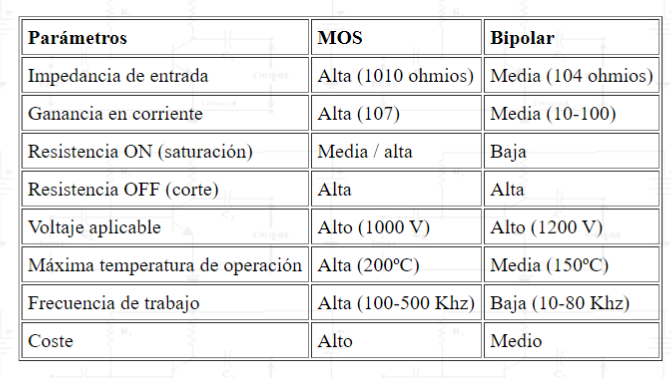
\includegraphics[scale=.70]{Parametros .png}\\
\raggedright
El IGBT ofrece a los usuarios las ventajas de entrada MOS, más la capacidad de carga en corriente de los transistores bipolares:\\
\bigskip
1.Trabaja con tensión.\\
2.Tiempos de conmutación bajos.\\
3.Disipación mucho mayor (como los bipolares).\\
\bigskip
Nos interesa que el transistor se parezca, lo más posible, a un elemento ideal:\\
\bigskip
1.Pequeñas fugas.\\
2.Alta potencia.\\
3.Bajos tiempos de respuesta (ton , toff), para conseguir una alta frecuencia de funcionamiento.\\
4.Alta concentración de intensidad por unidad de superficie del semiconductor.\\
5.Que el efecto avalancha se produzca a un valor elevado ( VCE máxima elevada).\\
6.Que no se produzcan puntos calientes (grandes di/dt ).\\
\bigskip
Una limitación importante de todos los dispositivos de potencia y concretamente de los transistores bipolares, es que el paso de bloqueo a conducción y viceversa no se hace instantáneamente, sino que siempre hay un retardo (ton,toff). Las causas fundamentales de estos retardos son las capacidades asociadas a las uniones colector - base y base - emisor y los tiempos de difusión y recombinación de los portadores.
\section{Principios básicos de funcionamiento}
La diferencia entre un transistor bipolar y un transistor unipolar o FET es el modo de actuación sobre el terminal de control. En el transistor bipolar hay que inyectar una corriente de base para regular la corriente de colector, mientras que en el FET el control se hace mediante la aplicación de una tensión entre puerta y fuente. Esta diferencia vienen determinada por la estructura interna de ambos dispositivos, que son substancialmente distintas.\\
\bigskip
Es una característica común, sin embargo, el hecho de que la potencia que consume el terminal de control (base o puerta) es siempre más pequeña que la potencia manejada en los otros dos terminales.\\
\bigskip
En resumen, destacamos tres cosas fundamentales:\\
1.En un transistor bipolar IB controla la magnitud de IC.\\
2.En un FET, la tensión VGS controla la corriente ID.\\
3.En ambos casos, con una potencia pequeña puede controlarse otra bastante mayor.\\
\section{Tiempos de conmutación}
Cuando el transistor está en saturación o en corte las pérdidas son despreciables. Pero si tenemos en cuenta los efectos de retardo de conmutación, al cambiar de un estado a otro se produce un pico de potencia disipada, ya que en esos instantes el producto IC x VCE va a tener un valor apreciable, por lo que la potencia media de pérdidas en el transistor va a ser mayor. Estas pérdidas aumentan con la frecuencia de trabajo, debido a que al aumentar ésta, también lo hace el número de veces que se produce el paso de un estado a otro.\\
\bigskip
Podremos distinguir entre tiempo de excitación o encendido (ton) y tiempo de apagado (toff). A su vez, cada uno de estos tiempos se puede dividir en otros dos.\\
\bigskip
Tiempo de retardo (Delay Time, td): Es el tiempo que transcurre desde el instante en que se aplica la señal de entrada en el dispositivo conmutador, hasta que la señal de salida alcanza el 10\% de su valor final.\\
\bigskip
Tiempo de subida (Rise time, tr): Tiempo que emplea la señal de salida en evolucionar entre el 10\% y el 90\% de su valor final.\\
\bigskip
Tiempo de almacenamiento (Storage time, ts): Tiempo que transcurre desde que se quita la excitación de entrada y el instante en que la señal de salida baja al 90\% de su valor final.\\
\bigskip
Tiempo de caída (Fall time, tf): Tiempo que emplea la señal de salida en evolucionar entre el 90\% y el 10\% de su valor final.\\
\bigskip
\centering
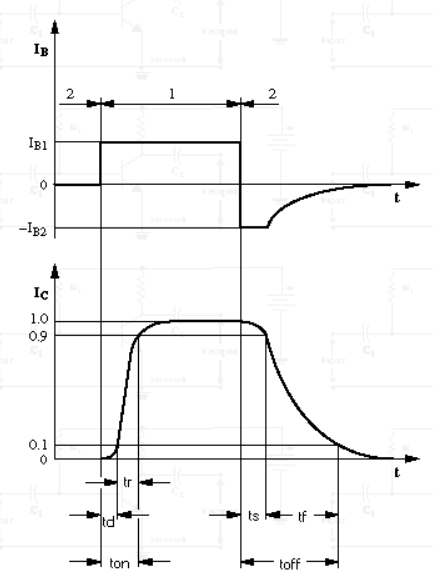
\includegraphics[scale=.70]{graf.png}\\
\raggedright
Es de hacer notar el hecho de que el tiempo de apagado (toff) será siempre mayor que el tiempo de encendido (ton).\\
Los tiempos de encendido (ton) y apagado (toff) limitan la frecuencia máxima a la cual puede conmutar el transistor:


\section{Otros parámetros importantes}
Corriente media: es el valor medio de la corriente que puede circular por un terminal (ej. ICAV, corriente media por el colector).\\
\bigskip
Corriente máxima: es la máxima corriente admisible de colector (ICM) o de drenador (IDM). Con este valor se determina la máxima disipación de potencia del dispositivo.\\
VCBO: tensión entre los terminales colector y base cuando el emisor está en circuito abierto.\\
VEBO: tensión entre los terminales emisor y base con el colector en circuito abierto.\\
\bigskip
Tensión máxima: es la máxima tensión aplicable entre dos terminales del dispositivo (colector y emisor con la base abierta en los bipolares, drenador y fuente en los FET).\\
\bigskip
Estado de saturación: queda determinado por una caída de tensión prácticamente constante. VCEsat entre colector y emisor en el bipolar y resistencia de conducción RDSon en el FET. Este valor, junto con el de corriente máxima, determina la potencia máxima de disipación en saturación.\\
\bigskip
Relación corriente de salida - control de entrada: hFE para el transistor bipolar (ganancia estática de corriente) y gds para el FET (transconductancia en directa).

\section{Modos de trabajo}
Existen cuatro condiciones de polarización posibles. Dependiendo del sentido o signo de los voltajes de polarización en cada una de las uniones del transistor pueden ser :\\
\centering
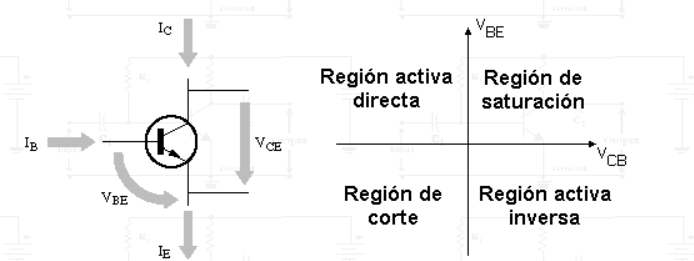
\includegraphics[scale=.80]{traba.png}\\
\raggedright
Región activa directa: Corresponde a una polarización directa de la unión emisor - base y a una polarización inversa de la unión colector - base. Esta es la región de operación normal del transistor para amplificación.\\
\bigskip
Región activa inversa: Corresponde a una polarización inversa de la unión emisor - base y a una polarización directa de la unión colector - base. Esta región es usada raramente.\\
\bigskip
Región de corte: Corresponde a una polarización inversa de ambas uniones. La operación en ésta región corresponde a aplicaciones de conmutación en el modo apagado, pues el transistor actúa como un interruptor abierto (IC 0).\\
\bigskip
Región de saturación: Corresponde a una polarización directa de ambas uniones. La operación en esta región corresponde a aplicaciones de conmutación en el modo encendido, pues el transistor actúa como un interruptor cerrado (VCE 0).\\
\section{Ataque y protección del transistor de potencia}
Como hemos visto anteriormente, los tiempos de conmutación limitan el funcionamiento del transistor, por lo que nos interesaría reducir su efecto en la medida de lo posible.\\
\centering
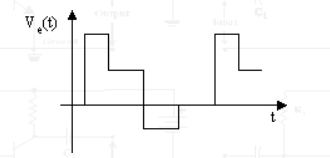
\includegraphics[scale=1]{s.png}\\
\raggedright
Los tiempos de conmutación pueden ser reducidos mediante una modificación en la señal de base, tal y como se muestra en la figura anterior.\\
Puede verse como el semiciclo positivo está formado por un tramo de mayor amplitud que ayude al transistor a pasar a saturación (y por tanto reduce el ton) y uno de amplitud suficiente para mantener saturado el transistor (de este modo la potencia disipada no será excesiva y el tiempo de almacenamiento no aumentará). El otro semiciclo comienza con un valor negativo que disminuye el toff, y una vez que el transistor está en corte, se hace cero para evitar pérdidas de potencia.\\
\bigskip
En consecuencia, si queremos que un transistor que actúa en conmutación lo haga lo más rápidamente posible y con menores pérdidas, lo ideal sería atacar la base del dispositivo con una señal como el de la figura anterior. Para esto se puede emplear el circuito de la figura siguiente.\\
\centering
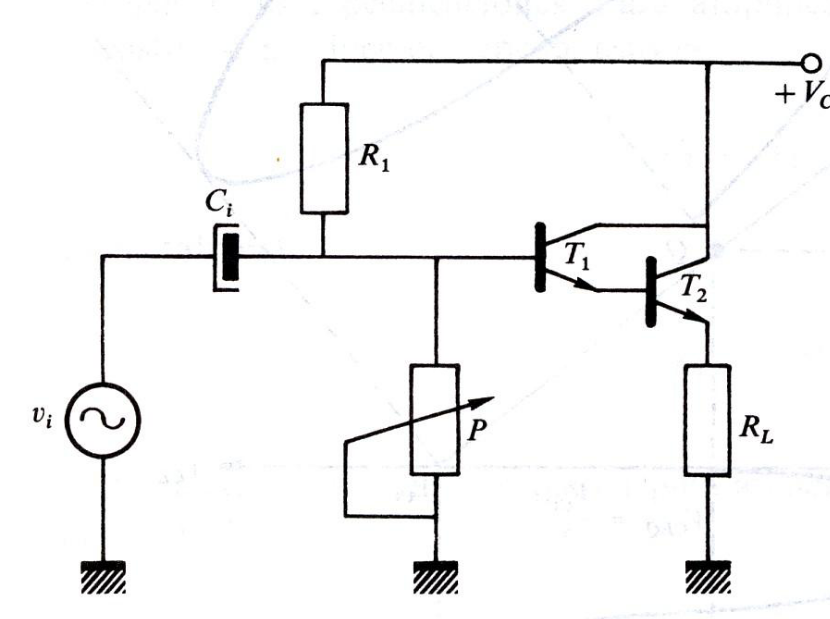
\includegraphics[scale=1]{cir.png}\\
\raggedright 
En estas condiciones, la intensidad de base aplicada tendrá la forma indicada a continuación:\\
\centering
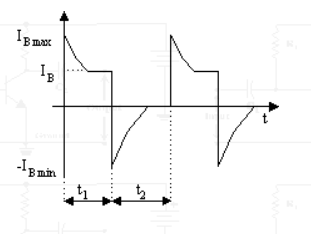
\includegraphics[scale=1]{te.png}\\
\raggedright
Durante el semiperiodo t1, la tensión de entrada (Ve) se mantiene a un valor Ve (máx). En estas condiciones la VBE es de unos 0.7 v y el condensador C se carga a una tensión VC de valor:\\
\centering
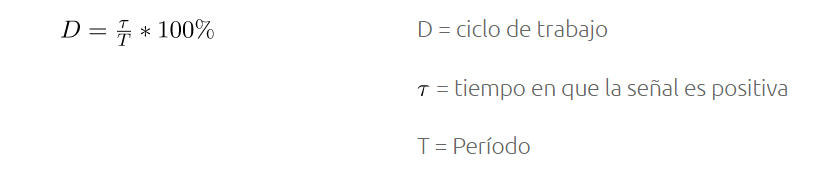
\includegraphics[scale=.70]{cal.png}\\ 
\raggedright
debido a que las resistencias R1 y R2 actúan como un divisor de tensión.\\
La cte. de tiempo con que se cargará el condensador será aproximadamente de:\\
\centering
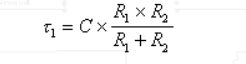
\includegraphics[scale=.70]{cal1.png}\\
\raggedright 
Con el condensador ya cargado a VC, la intensidad de base se estabiliza a un valor IB que vale:\\
\centering
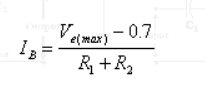
\includegraphics[scale=.70]{cal2.png}\\
\raggedright 
En el instante en que la tensión de entrada pasa a valer -Ve(min), tenemos el condensador cargado a VC, y la VBE=0.7 v. Ambos valores se suman a la tensión de entrada, lo que produce el pico negativo de intensidad IB (mín):\\
\centering
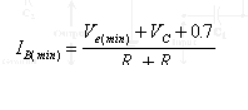
\includegraphics[scale=.70]{cal3.png}\\
\raggedright 
A partir de ese instante el condensador se descarga a través de R2 con una constante de tiempo de valor R2C.
\bigskip
Para que todo lo anterior sea realmente efectivo, debe cumplirse que:\\
\centering
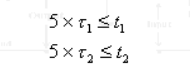
\includegraphics[scale=.70]{cal4.png}\\ 
\raggedright 
con esto nos aseguramos que el condensador está cargado cuando apliquemos la señal negativa. Así, obtendremos finalmente una frecuencia máxima de funcionamiento :\\
\centering
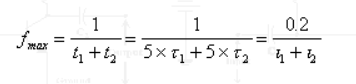
\includegraphics[scale=.70]{fmax.png}\\ 
\raggedright 
Un circuito más serio es el de Control Antisaturación:\\
\centering
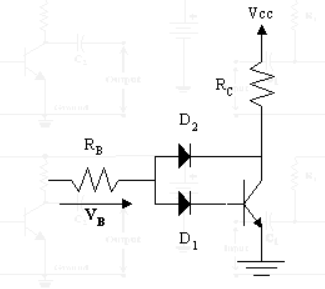
\includegraphics[scale=.80]{dia.png}\\
\raggedright 
El tiempo de saturación (tS)será proporcional a la intensidad de base, y mediante una suave saturación lograremos reducir tS :\\
\centering
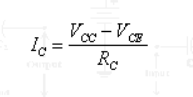
\includegraphics[scale=.70]{Ic.png}\\
\raggedright 
Inicialmente tenemos que:\\
\centering
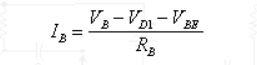
\includegraphics[scale=.70]{term.png}\\ 
\raggedright
En estas condiciones conduce D2, con lo que la intensidad de colector pasa a tener un valor:\\
\centering
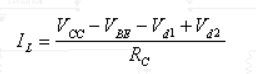
\includegraphics[scale=.70]{fina.png}\\ 
\raggedright
Si imponemos como condición que la tensión de codo del diodo D1 se mayor que la del diodo D2, obtendremos que IC sea mayor que IL:\\
\centering
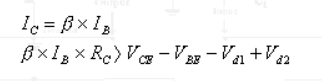
\includegraphics[scale=.70]{final.png}\\
\raggedright
\section{Referencias}
El Transistor en Circuitos de Potencia. Autor: Ing. Alberto C. Galiano\\
Circuitos de Potencia de Estado Sólido. Manual para proyectistas / SP-52 / RCA. Editorial Arbo.\\ 
\url{http://www.profesormolina.com.ar/electronica/componentes/transist/pot.htm}
\end{document}